% Compile directly from the doc directory.
% latexmk -xelatex -outdir=../build main.tex
\documentclass[acmsmall,screen,anonymous,review,nonacm]{acmart}
% Shared packages for the English manuscript.
\usepackage{amsmath}
\usepackage{listings}
\usepackage{algorithm}
\usepackage{algpseudocode}
\usepackage{subcaption}
\usepackage{tabularx}
\usepackage{flafter}

% Shared notation for path type contracts and state assertions.
\newcommand{\summary}[1]{\mathcal{S}_{#1}}
\newcommand{\contract}[3]{\left(#1,#2,#3\right)}
\newcommand{\typeat}[1]{\tau(#1)}
\newcommand{\ret}{\mathit{ret}}
\newcommand{\CanAdd}{\operatorname{CanAdd}}
\newcommand{\AddResult}{\operatorname{AddResult}}

% acmart already loads graphicx, xcolor, booktabs, and hyperref.
\graphicspath{{photos/}}
\algrenewcommand\algorithmicrequire{\textbf{Input:}}
\algrenewcommand\algorithmicensure{\textbf{Output:}}
\lstset{
  language=Python,
  basicstyle=\small\ttfamily,
  keywordstyle=\color{blue},
  commentstyle=\color{gray},
  numbers=left,
  numberstyle=\scriptsize,
  numbersep=6pt,
  breaklines=true,
  keepspaces=true,
  showstringspaces=false,
  columns=fullflexible,
  frame=tb,
  captionpos=b
}

\newcommand{\Aa}{\mathcal{A}}
\newcommand{\Bb}{\mathcal{B}}
\newcommand{\Cc}{\mathcal{C}}
\newcommand{\Mm}{\mathcal{M}}
\newcommand{\Tt}{\mathcal{T}}
\newcommand{\PSTC}{\mathit{PSTC}}

\newcommand{\jinlong}[1]{\color{red} {JL: #1 :LJ}\color{black}}
\newcommand{\yjw}[1]{\color{blue} { Y: #1 :Y }\color{black}}
\begin{document}
\title{Detecting Python Type Errors through Interprocedural Type-State Analysis}
\keywords{Python, type errors, type-state relations, interprocedural analysis,
  function summaries}
\begin{abstract}
Python type errors depend on the state in which an operation executes.
A function call can change the type of an object attribute or a global
variable, making a previously valid operation incompatible with the updated
state. Detecting such errors requires connecting input conditions to the
state changes established across calls. We present an interprocedural
type-state analysis for Python type-error detection. Its central model
relates function entries to ordered operation requirements, state updates,
and exits, preserving both conditional effects and intermediate failures.
The analysis constructs these relations by sharing facts independent of
unknown entry types and using a large language model to propose implicit
type alternatives. At each call, it instantiates object identities and
propagates the corresponding state changes. A conflict triggers selective
expansion of the relevant callee type paths and contextual re-inference;
revised relations then update dependent callers. The analysis separately
reports runtime type errors and annotation-contract errors. We evaluate
paired detection on xxx recent GitHub bug-fix records, diagnostic precision,
component effects, and total analysis cost. The evaluation reports
xxx paired runtime detections and xxx paired annotation-contract detections,
with respective diagnostic precision of xxx\% and xxx\%.
\end{abstract}

\maketitle

\section{Introduction}
\label{sec:introduction}

Python's dynamic type system allows variables to change type at
runtime and operations to accept different input types, offering
developers considerable flexibility.
However, this flexibility can also lead to subtle type errors
that remain undetected until runtime.
These errors can interrupt program
execution and cause application failures, compromising software
reliability.
Consequently, substantial effort has been devoted
to static type-error detection for Python, aiming to identify
such errors before execution.

In recent years, many studies have explored type-error detection for Python
code, encompassing both \textit{gradual-typing-based}~\cite{mypy,pyrefly,pyright}
and \textit{inference-based}~\cite{oh2024pyinder,rTED} approaches.
On the one hand, \textit{gradual-typing-based} approaches use type annotations
to check assignments, function calls, and other operations against declared
types and have been adopted in major production codebases and open-source
projects, including Dropbox, Instagram, PyTorch, and
JAX~\cite{dropboxMypy,pyreflyAdoption}.
On the other hand, \textit{inference-based} approaches automatically infer
the most likely types of parameters from their usage patterns,
using predefined similarity measures or LLMs, thereby enabling
type-error detection in repositories that lack type annotations.
These methods have demonstrated their effectiveness on standard benchmarks.
For example, on the widely used \textit{BugsInPy} and \textit{TypeBugs}
benchmarks~\cite{bugsinpy,typebugs}, existing methods achieve an accuracy of up to
50\% (34/68)~\cite{oh2024pyinder}, indicating the potential of current
techniques for type-error detection.
However, when applied to real-world Python repositories, which often 
involve complex type-transition in different execution paths, 
existing approaches face significant challenges. 
As illustrated in our preliminary study (see the motivating examples in Section~\ref{sec:background}), 
both types of approaches, as well as native LLMs, frequently fail to detect type errors in the 
presence of complex type-transition, particularly type-transition across function calls, 
which are commonly encountered in real-world codebases. 
This limitation underscores a persistent gap between current research and its 
applicability to real-world Python repositories.

To address this gap, we aim to propose a \textbf{type-transition-aware type error detection} approach.
Leveraging the superior semantic understanding capabilities of Large Language Models (LLMs), we
adopt LLMs as the core detection engine of our approach. Based on our investigation, we have
identified three key challenges to our approach.

\paragraph{Challenge 1: Modeling type-state changes across function calls.}
A function can change the type-state of call-site not only through its return
value but also by updating global variables or attributes of mutable
objects. 
These updates depend on the function's execution path, so calls
to the same function can establish different type-states. Conventional
type annotations describe parameter, return, and attribute types, but do
not specify how a call transforms the incoming type-state under different
execution conditions. We therefore need a new model to express these
conditional type-state changes and their effects on subsequent operations.

\paragraph{Challenge 2: Extracting conditional type-state changes from code.}
Program execution involves both explicit and implicit paths. Explicit
paths arise from branch statements, while implicit paths arise from Python
operations whose behavior depends on the types involved. For example,
addition can perform arithmetic, concatenate strings, or invoke a
user-defined method, with different type requirements and effects in each
case. Analyzing these paths across function calls further requires
considering combinations of caller and callee paths, leading to path
explosion. Accounting for implicit paths and managing path explosion
therefore make it challenging to extract conditional type-state changes
from code.

\paragraph{Challenge 3: Detecting type errors using conditional type-state changes.}
Due to limitations in analysis precision, the extracted type-state
transition relations may contain inaccuracies, which can cause valid
operations to be flagged as type errors. A detected type conflict therefore
does not necessarily indicate
an error in the program. Distinguishing a real error from an analysis
inaccuracy requires examining how the conflicting state arises under the
relevant calling conditions. Moreover, an inaccurate type-state change
can propagate through multiple calls, affecting error detection in other
functions. The challenge is therefore to distinguish type errors
from false alarms and correct analysis inaccuracies.

To address these challenges, we propose PyTT(Python Type Tracker), a Python type-error detector
that models and tracks conditional type-state transitions across function
calls. To address \textbf{Challenge 1}, we introduce a
\emph{path-sensitive type contract} (PSTC) to represent these transitions,
capturing a function's type requirements and updates along different
execution paths. To address \textbf{Challenge 2}, PyTT uses static analysis
to identify explicit paths and a large language model (LLM) to infer
implicit paths. It further uses static analysis to
simplify code whose type behavior is independent of the calling context,
reducing repeated analysis across paths to mitigate path explosion.
To address \textbf{Challenge 3}, PyTT uses PSTCs to trace detected conflicts
across function boundaries. It analyzes the resulting traces to distinguish
type errors from false alarms. For false alarms, PyTT corrects the
inaccuracies in the corresponding contracts and updates the affected
analysis results.

We evaluate PyTT on xxx real-world type-error fixes from xxx Python
repositories, measuring detection effectiveness, diagnostic precision,
and analysis cost. PyTT detects xxx runtime type errors and xxx
annotation-contract errors, with precision of xxx\% and xxx\%, respectively.
Each detection is checked against both the buggy and fixed revisions.
Ablation experiments examine the contributions of conditional type-state
modeling, explicit and implicit path analysis, and conflict analysis and
correction. We further evaluate PyTT on xxx independent repositories,
where it identifies xxx previously unknown type errors.

The contributions are as follows:
\begin{itemize}
  \item We introduce the path-sensitive type contract (PSTC), a model
  that captures conditional type-state transitions across function calls
  for Python type-error detection.
  \item We propose PyTT, a type-error detection method that combines
  static analysis and LLM-based analysis to extract these transitions.
  PyTT analyzes conflict traces across functions to distinguish type
  errors from false alarms and correct analysis inaccuracies.
  \item We evaluate PyTT on real-world type-error fixes and independent
  Python repositories, assessing detection effectiveness, diagnostic
  precision, and analysis cost, and examining the contributions of its
  key components through ablation experiments.
\end{itemize}

\section{Background and Motivating Example}
\label{sec:background}

% [M1]
In this section, we explain how dynamic typing and duck typing in Python
affect type-error detection. We then introduce Hoare triples and explain
how their preconditions and postconditions can summarize function behavior.

\subsection{Dynamic Typing and Duck Typing in Python}

% [M2]
A type-error detector must determine which types an operation's operands
can have and check whether the operation supports those
types~\cite{oh2024pyinder}. Python's dynamic typing and duck typing
complicate these tasks. With dynamic typing, the values used by an
operation may have different types on different executions.
Under duck typing, objects of different classes can support the same
operation. To check compatibility, a detector must examine whether the
operands meet the requirements of the methods or protocols used by that
operation. Moreover, the same operation may invoke different
implementations for different operand types. These implementations may
return values of different types, affecting the types used by subsequent
operations.

% [M3]
More specifically, \textbf{dynamic typing} allows both local and global
variables in Python to be bound to objects of different
types during program execution~\cite{pythonExecutionModel,pythonDataModel}.
Consequently, an operand's type depends on the assignments and updates
along the execution path to the operation.
% [M4]
Function calls can also change the values that a caller uses. A caller may
assign a function's return value to a variable. A callee may also update a
global variable or an attribute of an object shared with its caller.
When the caller next reads the updated variable or attribute, it may
obtain a value of a different type, even if the callee did not return that
value. To determine the types used by subsequent operations, a detector
must therefore track assignments and updates both within functions and
across calls.

% [M5]
In Python, code written in the \textbf{duck typing} style uses objects
through the methods and attributes they support, without requiring them
to belong to a particular class~\cite{pythonGlossary}.
For an operation that calls a method on an operand, a detector must check
that the object supports that method and that the call satisfies the
method's requirements.
% [M6]
Beyond checking whether an operation accepts its operands, a detector
must account for what its implementation returns or updates. Python's
dispatch rules may select different implementations for different operand
types. These implementations may return values of different types or
update state that subsequent operations read. The detector must track
these effects because later operations use the resulting values and
updated state.

% [M7]
To check subsequent operations precisely, a detector can relate the types
and state before each operation to its result and the state after it.
For a function call, this relation connects the argument types and the
types of shared values before the call to the return type and the types
of updated values after it. The shared values include global variables
and object attributes that the function reads or updates.
The same function may return or update values of different types under
different calling conditions or along different execution paths. If the
detector records only the possible resulting types, it loses the
conditions under which each type arises. It may then consider types that
cannot occur in the current calling context when checking a later
operation. Keeping each result associated with its conditions allows the
detector to use the type information relevant to that call.

\subsection{Hoare Triples as Function Summaries}
\label{sec:hoare-background}

% [M8]
To check operations after a call, a detector must account for the values
returned or updated by the callee. A function summary describes the
callee's relevant behavior so that the detector can reuse it at call
sites. For type-error detection, a summary can relate conditions on the
arguments and shared state before the call to type facts that hold after
it returns normally. Hoare triples provide a standard way to express
this relationship between conditions before and after execution.

Hoare logic describes how executing a program changes its
state~\cite{hoare1969axiomatic,softwareFoundationsHoare}. A Hoare triple has
the form
\begin{equation}
\{P\}\ C\ \{Q\},
\label{eq:hoare-triple}
\end{equation}
% [M9]
where $C$ is a command, and $P$ and $Q$ are assertions over program states,
called the precondition and postcondition, respectively. An assertion
describes a property of a state, such as the type of a value held in a
variable.
% [M10]
We use a partial-correctness interpretation that describes what holds on
normal termination. A valid triple states that if $P$ holds before $C$
executes and $C$ terminates normally, then $Q$ holds afterward. In other
words, $P$ gives the assumptions under which executing $C$ establishes $Q$
on normal termination. Under this interpretation, the triple does not
guarantee that $C$ terminates or executes without raising a
\texttt{TypeError}.

% [M11]
When a Hoare triple is used as a function summary, its precondition can
express assumptions about the arguments and shared state, while its
postcondition can describe the return value and properties of the shared
state after the call.
% [M12]
To apply the summary at a call site, the detector matches the callee's
parameters with the caller's arguments and interprets references to
shared objects in the caller's state. This step instantiates the summary
for the call. If the calling state satisfies the instantiated
precondition, the postcondition gives facts that hold when the call
returns normally. The detector can use these facts to check subsequent
operations. If the calling state does not satisfy the precondition, the
detector cannot rely on this guarantee. That alone does not establish a
type error. To determine whether an error occurs, the detector must
examine the relevant operations and their exceptional behavior.

% [M13]
Hoare triples also support sequential composition. If
$\{P\}\ C_1\ \{R\}$ and $\{R\}\ C_2\ \{Q\}$ are valid, then
$\{P\}\ C_1; C_2\ \{Q\}$ is valid. Here, $R$ is an intermediate assertion.
Starting from a state satisfying $P$, $C_1$ establishes $R$ on normal
termination. This assertion then serves as the precondition for the
second triple. Thus, the properties established by
one command provide the assumptions for reasoning about the next command.

% [M14]
For Python type-error detection, a detector can use a function summary to
update the type facts it uses after a call. If a function updates an
attribute of a shared object, its postcondition can describe the type of
the value held in that attribute on normal return. The caller still
accesses the same object, but the attribute now holds the updated value.
A type fact about its previous contents may therefore no longer apply.
The detector must check subsequent operations using type facts that
account for the update. When the calling state satisfies the summary's
precondition, its postcondition can provide these facts.

% [R01]
\subsection{Motivating Example}
\label{sec:motivating-example}

% [R02]
Figure~\ref{fig:motivating-example} presents a message-processing
example that illustrates the need to track type-state changes across
function calls. The function \texttt{make\_line} calls
\texttt{encode\_message} to encode a message body before appending
a newline. The body is declared as \texttt{str | bytes}.
For a string body, \texttt{encode\_message} invokes the supplied
encoder and stores its result in the same message object.
\texttt{TextEncoder} returns the string unchanged, whereas
\texttt{Utf8Encoder} converts it to bytes.

% [R02a]
As shown in the figure, Mypy, Pyrefly, and Pyright do not report the
concatenation error, whereas PyTT detects it. Analyzing this example
reveals two related requirements for type-error detection. First,
the analyzer must propagate changes to the shared message body across
the call so that the subsequent operation is checked against its
updated type. Second, distinguishing the failing UTF-8 call from the
safe text-encoder call requires retaining the conditions under which
each update occurs. We examine these requirements below and explain
how PyTT addresses them through conditional type-state summaries.

\begin{figure}[!htbp]
\centering
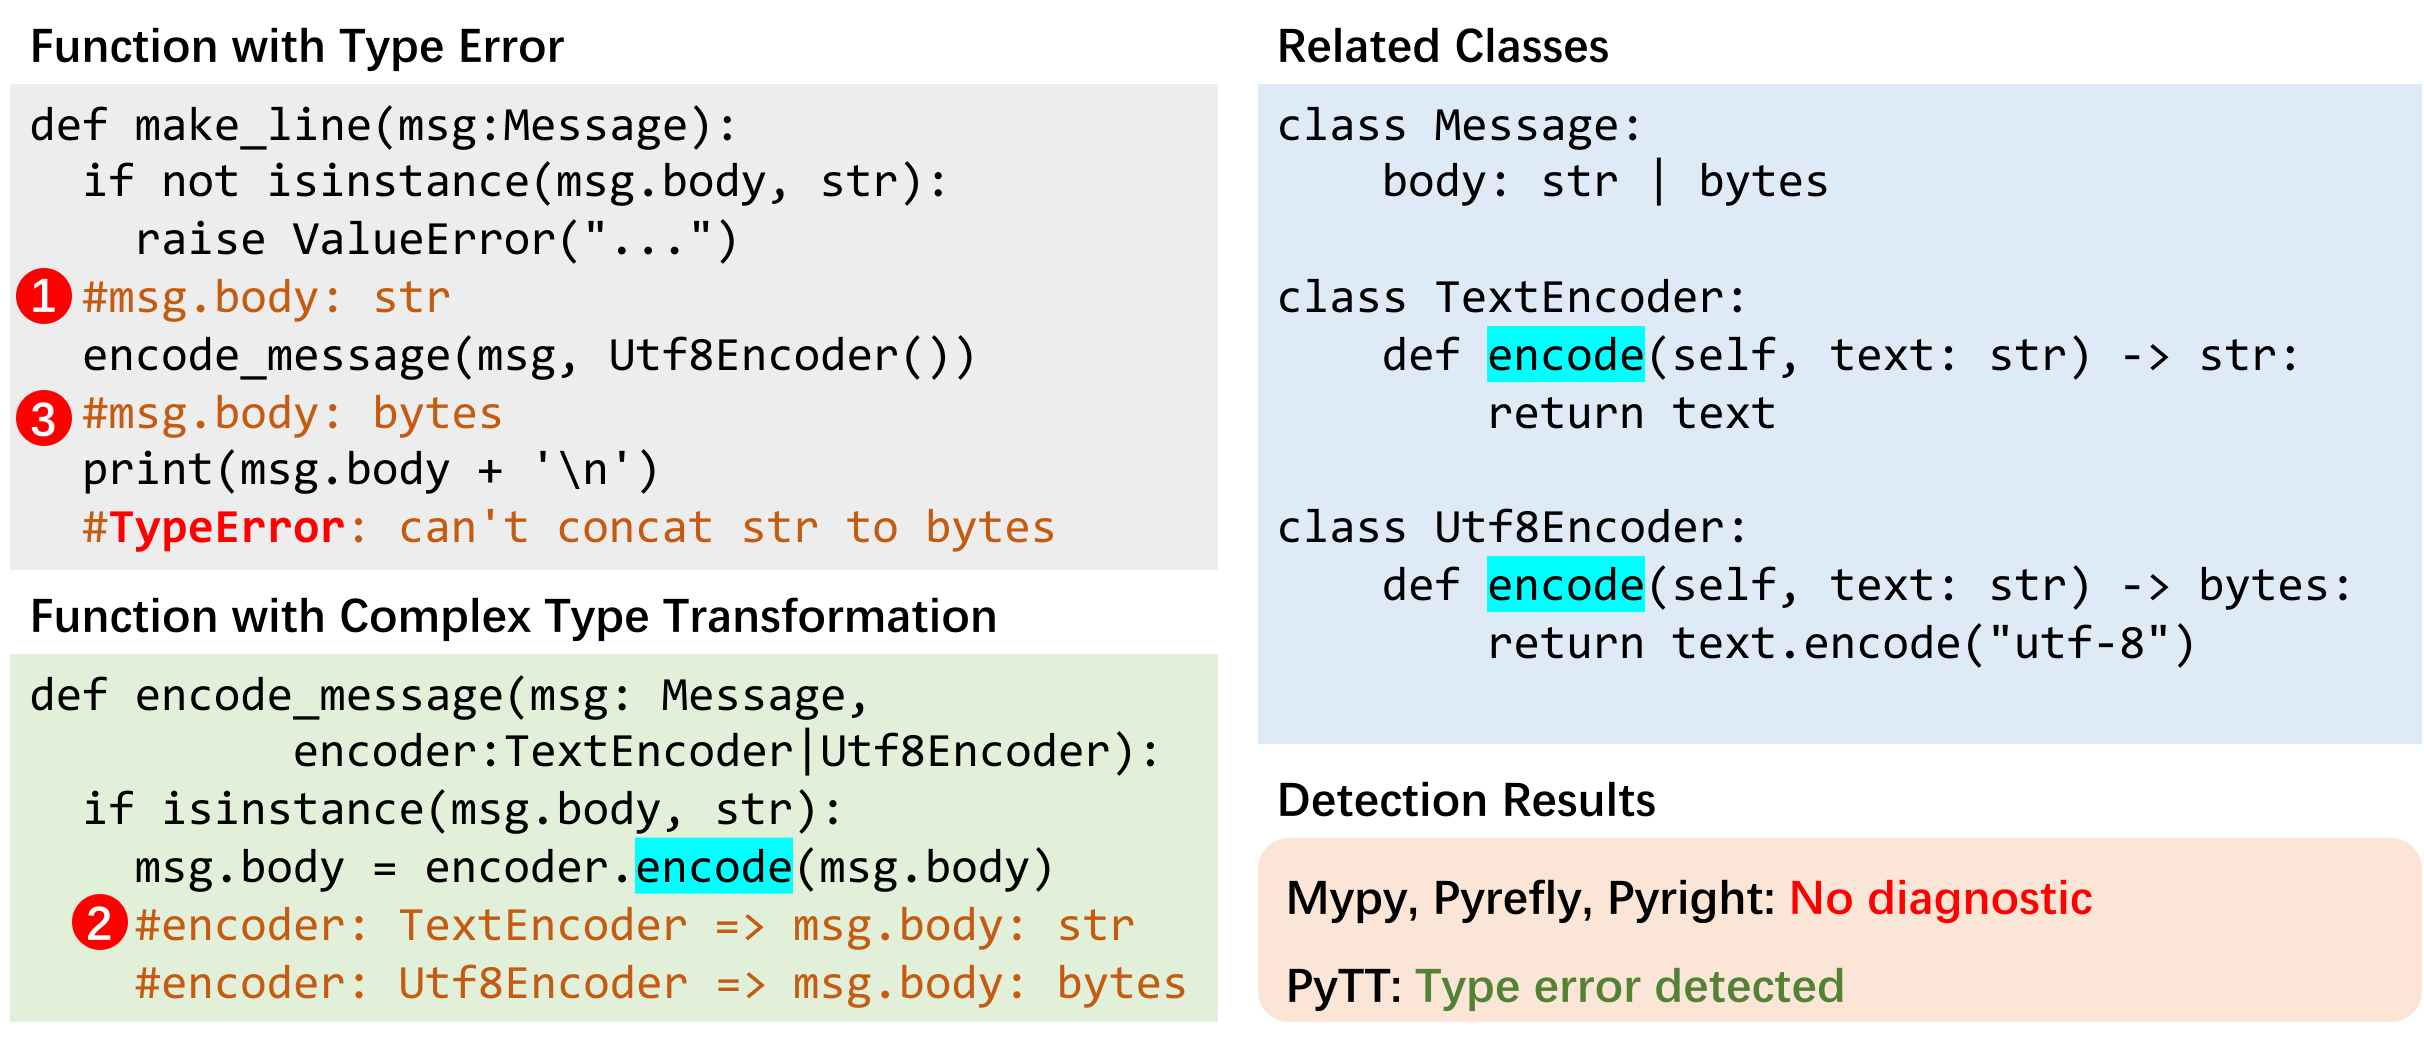
\includegraphics[width=\linewidth]{photos/motivatingExample.png}
% [R03]
\caption{Motivating example of interprocedural type-state changes
and type-error detection results.}
\Description{The caller make_line rejects a non-string message body,
then calls encode_message with Utf8Encoder and attempts to concatenate
msg.body with a newline string. For a string input, the helper writes
the encoder's result into the same message object. TextEncoder returns
a string, and Utf8Encoder returns bytes. Points 1, 2, and 3 mark the
string body before the call, the conditional field updates, and the
bytes body after the UTF-8 call returns normally. The concatenation
then raises TypeError. The result panel labels Mypy, Pyrefly, and
Pyright with No diagnostic and PyTT with Type error detected.}
\label{fig:motivating-example}
\end{figure}

% [R04]
\textbf{(1) Interprocedural Type-State Propagation.}
In \texttt{make\_line}, the guard raises \texttt{ValueError} when
\texttt{msg.body} is not a string. Thus, the body has type
\texttt{str} at point~1. The subsequent call passes \texttt{msg}
and a \texttt{Utf8Encoder} instance to \texttt{encode\_message},
which writes the encoding result into \texttt{msg.body}. Because
both functions access the same message object, the body has type
\texttt{bytes} at point~3 after the call returns normally.
The expression \texttt{msg.body + '\textbackslash n'} then raises
\texttt{TypeError} before \texttt{print} is invoked, and the exception
escapes \texttt{make\_line}.

% [R05]
Both the original string and the updated bytes satisfy the field's
union annotation, but the updated body does not support concatenation
with a string. Detecting this error requires propagating the field
update from \texttt{encode\_message} to its caller. The function's
return type, \texttt{None}, does not describe this update. If the
analyzer retains the string type established at point~1, it can miss
the error at point~3.

% [R06]
\textbf{(2) Conditional Type-State Modeling.}
Propagating a field update also requires determining which type the
call establishes. In this example, that type depends on the encoder
argument. Replacing \texttt{Utf8Encoder} with
\texttt{TextEncoder} leaves a string body and makes the concatenation
valid. An analyzer that assigns \texttt{str | bytes} to the body
after either call can flag the potential bytes/string conflict.
However, retaining the bytes alternative for \texttt{TextEncoder}
can also cause a false alarm. Distinguishing these calls therefore
requires preserving the relation between the encoder argument and the
resulting field type under the incoming string condition.

% [R07]
PyTT addresses these requirements using path-sensitive type contracts
(PSTCs), which record field updates together with their calling
conditions and propagate the applicable updates to callers. At point~2,
the contract for \texttt{encode\_message} records two cases for an
incoming string body. On normal return, the \texttt{TextEncoder}
case establishes a string body, and the \texttt{Utf8Encoder} case
establishes a bytes body. For a non-string input, the function leaves
the body unchanged.

% [R08]
At the illustrated call, PyTT uses the string type established by the
guard and the \texttt{Utf8Encoder} argument to select the second case.
It maps the callee's message parameter to the caller's object and
updates the type of \texttt{msg.body} accordingly. The subsequent
concatenation is therefore checked with a bytes body, revealing the
type error.


\section{Approach}
\label{sec:method}

This section introduces our solution for \textit{"how to perform type-transition-aware type error detection"}.

\subsection{Overview}

\begin{figure}[!htbp]
\centering
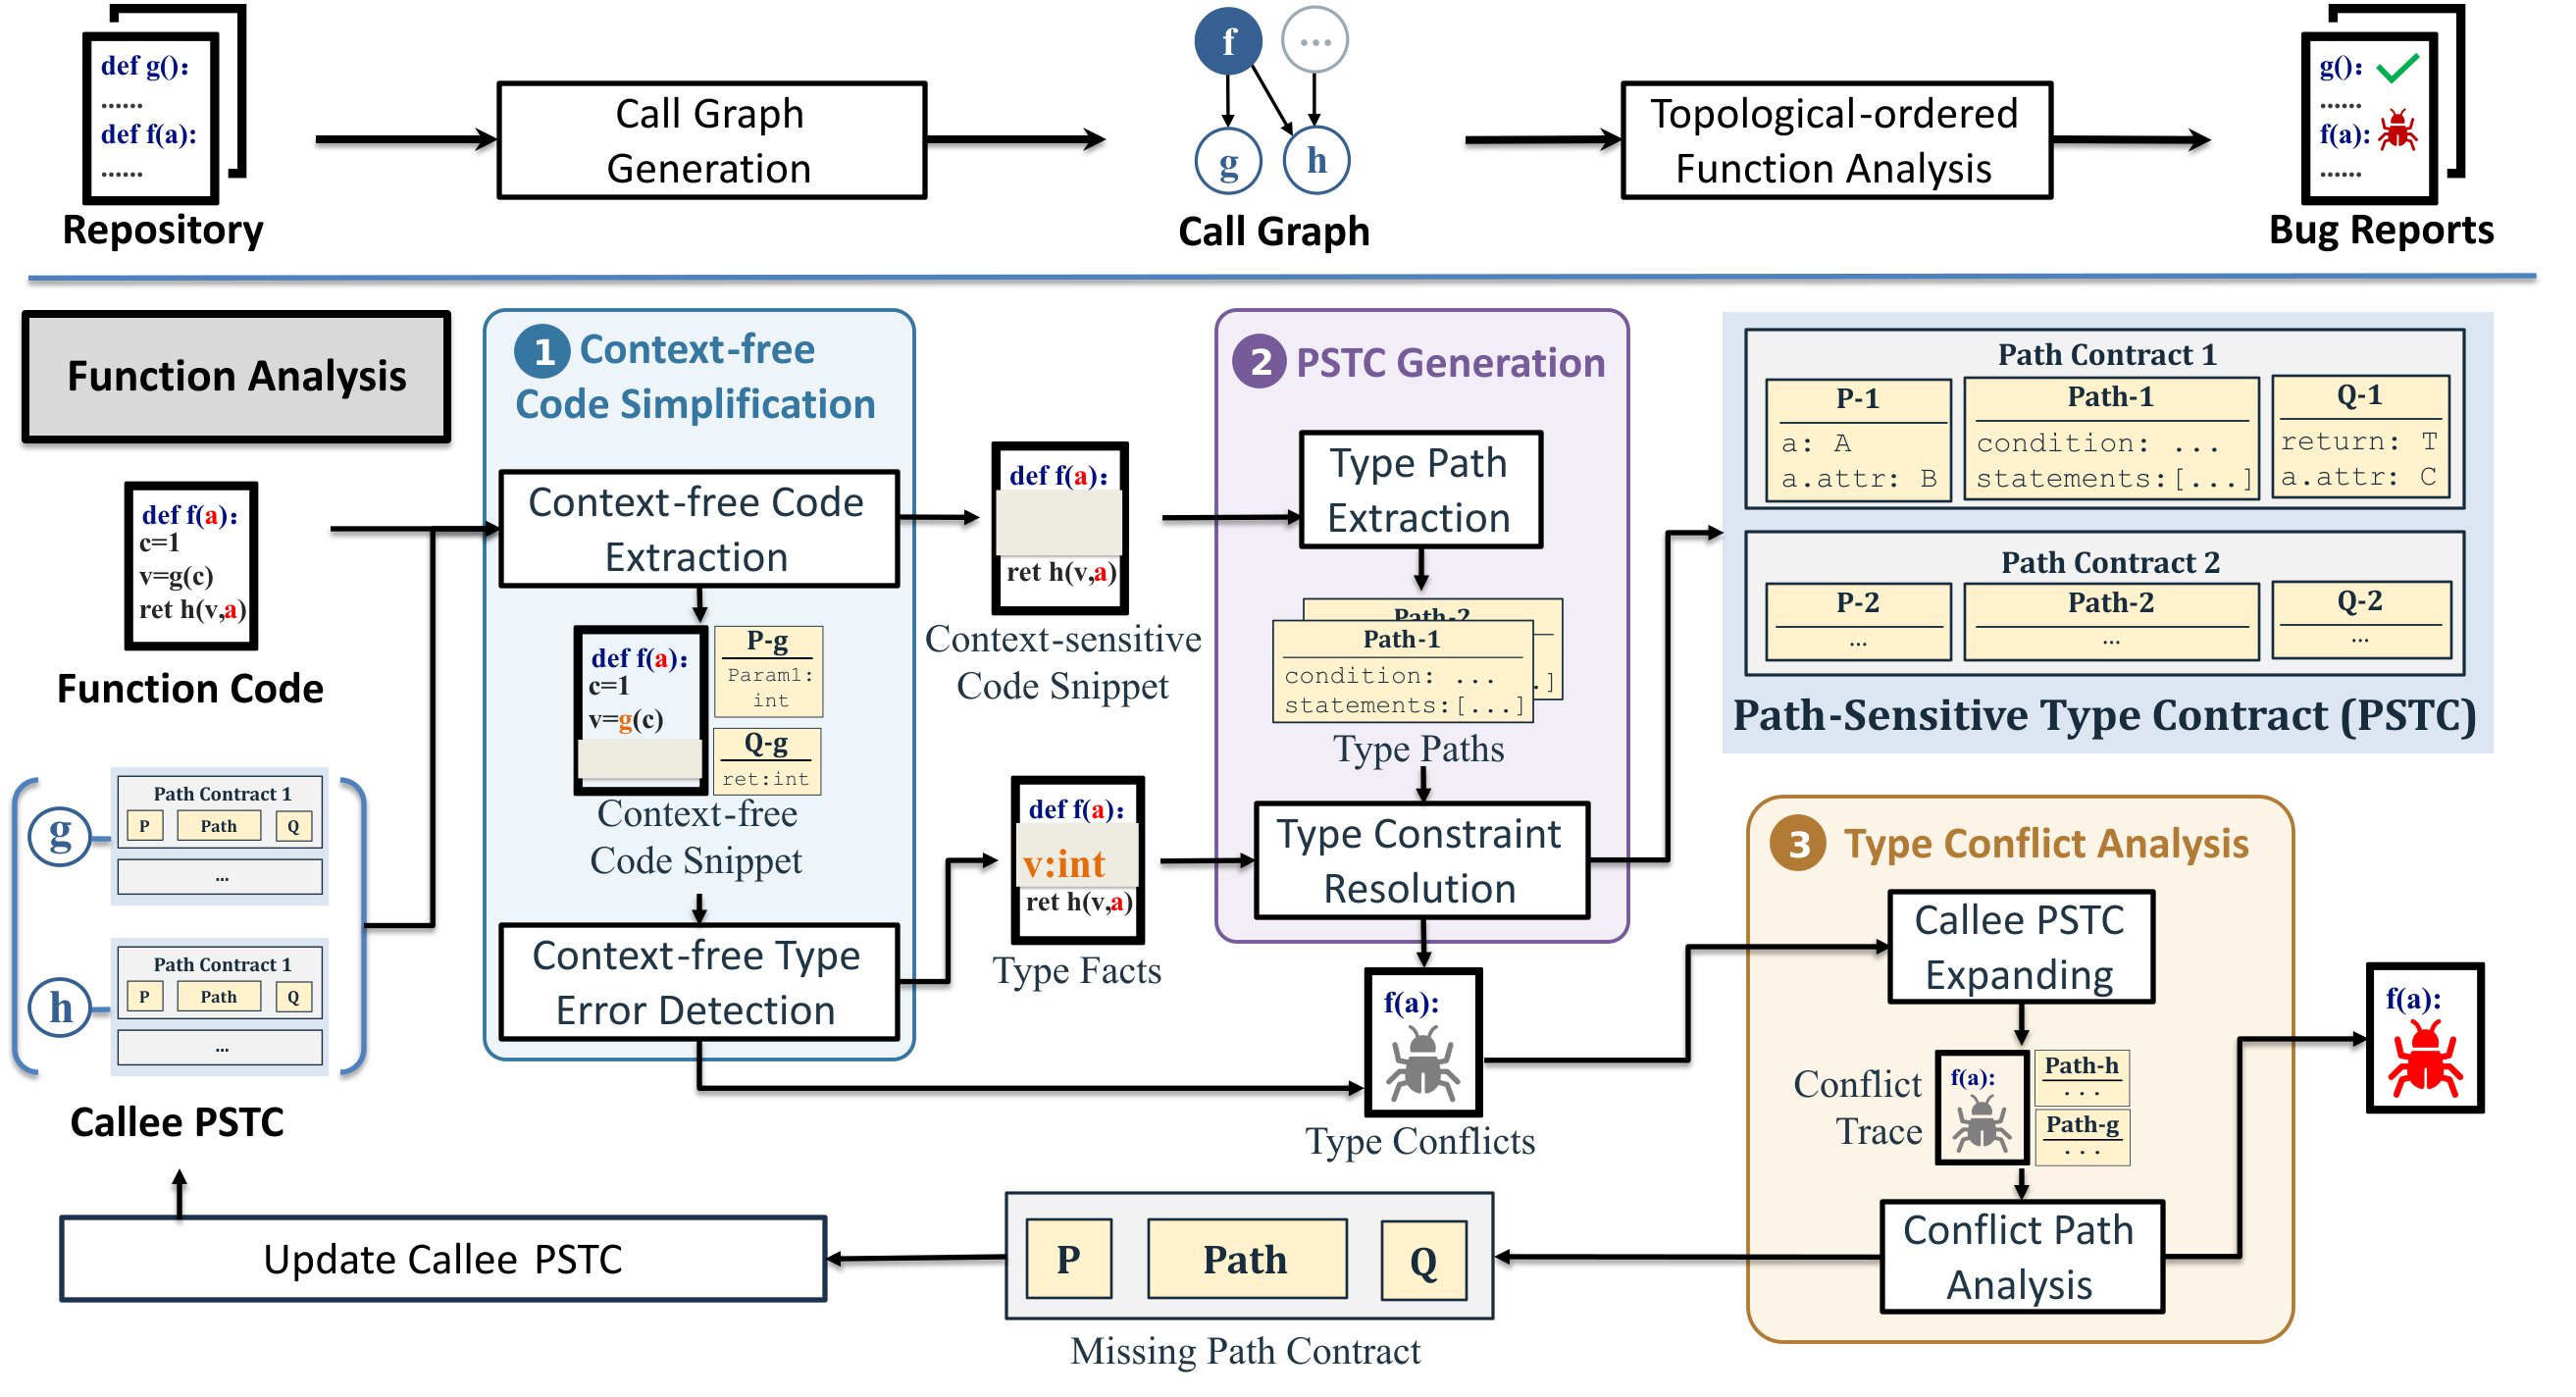
\includegraphics[width=\linewidth]{photos/methodOverview.png}
\caption{Overview of PyTT's workflow}
\label{fig:method-overview}
\end{figure}


Figure~\ref{fig:method-overview} illustrates the workflow of PyTT for type-transition-aware type error detection. 
PyTT processes functions in a callee-before-caller topological order over the call graph. 
For each function, it detects type errors within the function and constructs a 
\emph{path-sensitive type contract} (PSTC) that summarizes the function's type transitions along different execution paths. 
The resulting PSTC is propagated to callers to support interprocedural analysis. 
Specifically, PyTT analyzes each function in three phases.

\textbf{(1) Context-free Code Simplification}. 
To check the uses of variables with known types and prune unnecessary paths, PyTT performs type checking and simplification on code whose type behavior is independent of the function's inputs.
PyTT identifies variables whose types are independent of the function's inputs and uses static analysis to trace their propagation, thereby extracting the context-free code.
It then leverages an LLM to check whether these variables are used correctly and simplifies the extracted code into type information for expressions used in the context-sensitive code, supporting subsequent analysis of that code.

\textbf{(2) PSTC Generation}.
In this phase, PyTT analyzes the remaining context-sensitive code to construct a PSTC that captures the function's type transitions under different execution conditions.
PyTT first identifies explicit execution paths within the context-sensitive code through static analysis.
For each explicit path, PyTT uses an LLM to derive behavioral constraints on the inputs and infer the possible input type-states that satisfy these constraints, thereby identifying distinct implicit paths.
Each path, together with its input and output type-states, forms a path contract, and these contracts collectively constitute the function's PSTC.
Additionally, behavioral constraints that admit no valid input type-state indicate conflicting requirements on the behavior of the variables and are also identified as type errors.

\textbf{(3) Type Conflict Analysis}.
To distinguish type errors from false alarms caused by inaccurate PSTCs, 
PyTT examines the source behavior underlying each detected type conflict.
Once a type conflict is detected, PyTT uses the path recorded in the callee's PSTC 
to trace the conflicting type facts through the relevant caller and callee code.
The type transitions along the resulting interprocedural path are re-inferred using an LLM.
If this analysis confirms a type error, PyTT reports it together with the confirmed interprocedural trace that triggers the error.
Otherwise, the analysis reveals an inaccurate PSTC, which PyTT corrects to dismiss the resulting false alarm.

Following a callee-before-caller topological order over the call graph, 
PyTT first simplifies each function into a context-sensitive code 
snippet in the \textit{Context-free Code Simplification} phase.
The \textit{PSTC Generation} phase then summarizes the type 
transitions along different paths into a PSTC, 
providing interprocedural type-transition information for type error detection in callers.
The PSTC is corrected and updated through the \textit{Type Conflict Analysis} phase.
Once all functions in the repository have been analyzed along the call chains, 
PyTT collects all detected type errors and compiles them into an error report for the repository.

\subsection{Design of Path-Sensitive Type Contracts}
\label{sec:state-model}


The motivating example establishes two requirements for a function
summary. It must describe the change of type to values shared with the caller, and
it must retain the conditions under which each change occurs. 
PyTT therefore needs a summary that connects the incoming type-state and
execution conditions to the types established by the call.

Before defining the contract, we introduce the abstraction that it
relates. 
A \emph{type-state} is a simplified form of program state. It
abstracts away from the concrete values that a program manipulates and
retains only the type information required by the checks of subsequent
operations. At a program point, a type-state describes the type of a
parameter, a local or global variable, or a class or instance attribute.
At point~1 of Figure~\ref{fig:motivating-example}, for example, the
type-state records that the message body holds a string. Because a
function can be called under different type-states, PyTT describes its
behavior as a relation between the type-states at its entry and its exit,
rather than in terms of particular values.


  \begin{definition}[Path-sensitive Type Contract (PSTC)]
  For a function $\Mm$, its path-sensitive type contract is
  \[
      \Cc \subseteq \Aa_{\Mm} \times \Mm \times \Aa_{\Mm},
  \]
  where $\Aa_{\Mm}$ is the set of assertions among the \textit{type-states} of the
  variables related to $\Mm$.
  Each $c=(p,m,q)\in\Cc$ is a path contract representing the type transition on a specific execution path, where
  \begin{itemize}
    \item $p\in\Aa_{\Mm}$ is the entry assertion, describing the type-state required at entry to the function; 
    \item $m\in\Mm$ is the path description, recording the guards, operation requirements, calls, and updates along one execution path in execution order; 
    \item $q\in\Aa_{\Mm}$ is the exit assertion, describing the type-state and the return value established when that path returns normally. 
  \end{itemize}
  % Different cases of a function describe the type-state changes established under different entry conditions and execution paths.
  \end{definition}


Take the function \texttt{encode\_message} in
Figure~\ref{fig:motivating-example} as an example.
Besides the explicit path condition on the type of
\texttt{msg.body}, duck typing introduces implicit path
conditions on the \texttt{encoder} argument: the same encoder call
invokes different implementations depending on its type.
The PSTC of \texttt{encode\_message} therefore contains three
path contracts in this example.
Consider $c_{\mathrm{utf8}}=(p_{\mathrm{utf8}},
m_{\mathrm{utf8}},q_{\mathrm{utf8}})$, whose entry assertion is
\[
p_{\mathrm{utf8}} =
\{ \texttt{msg}:\texttt{Message},\;
   \texttt{msg.body}:\texttt{str},\;
   \texttt{encoder}:\texttt{Utf8Encoder} \}.
\]
This assertion combines the explicit condition about \texttt{msg.body}
with the implicit condition about \texttt{encoder} argument. 
The path description $m_{\mathrm{utf8}}$ records, in execution
order, the successful string test, the encoder call that
converts the string to bytes, and the assignment of those
bytes to \texttt{msg.body}.
The exit assertion is
\[
q_{\mathrm{utf8}} =
\{ \texttt{ret}:\texttt{None},\;
   \texttt{msg.body}:\texttt{bytes} \},
\]
where \texttt{ret} denotes the function's return value.
Although the function returns \texttt{None}, this assertion
captures the updated type of the shared field.
At the illustrated call, this contract connects the
string-body type-state at point~1 to the bytes-body
type-state at point~3 through the update at point~2.
The second contract requires a string body and a
\texttt{TextEncoder} argument, records the encoder call
and assignment, and establishes a \texttt{str} body on return.
The third contract covers the non-string branch, on which
the encoder is not called and the body type remains unchanged.
Together, these contracts form $\Cc$, preserving the
association between each entry assertion, the corresponding
execution path, and its resulting type-state.


\subsection{Phase I: Context-free Code Simplification}
\label{sec:extraction}

Constructing the contract defined above requires examining behavior under
different entry conditions and execution paths.
When a path contains calls, its analysis also depends on the relevant
paths of the callees, increasing the number of combinations to consider.
Our insight is that PSTC construction only requires exploring the
context-sensitive portion of a function under different entry conditions.
Context-free paths and calls can be checked and simplified using known
types, without propagating their internal paths across function boundaries.
Accordingly, PyTT first extracts the context-free code from the function
under analysis and uses an LLM to check its type correctness.
It also simplifies this code into type information for expressions used
by the context-sensitive code, allowing subsequent analysis to reuse
these facts without reexamining the corresponding computations.


\subsubsection{Context-free Code Extraction}

To identify code whose type behavior is independent of the entry
type-state, PyTT traces the propagation of known types along def-use
chains.
Starting from expressions whose types are determined by local semantics
or available callee PSTCs, it identifies statements whose expressions
can all be resolved using these types.
The types of local variables defined by these statements are then propagated
to identify further context-free expressions and statements.
When these statements are control-dependent on the function's inputs,
PyTT separates the corresponding branches into distinct paths and
performs this extraction within each path.
The resulting statements form the context-free code under their
respective path conditions.

For a function call expression, this extraction relies on the callee's
PSTC to determine the return type.
If the PSTC contains a single path with an input-independent return
type, PyTT directly treats the return value as context-free.
Otherwise, PyTT checks whether the callee's entry type-state can be
determined from context-free expressions at the call site.
If so, it uses the known types to select the applicable path contracts
and infer the possible return types.
If neither condition holds, the return type depends on unresolved
input types, and the call remains context-sensitive.

For a statement containing both context-free and context-sensitive
expressions, PyTT extracts its maximal context-free subexpressions.
Their types will be inferred and recorded when checking the context-free
code, then supplied to the analysis of the enclosing statement.
This allows subsequent analysis to focus on the context-sensitive
expressions without reexamining the context-free parts.

Consider a function \texttt{f(s)} that calls
\texttt{data = json.loads(s)} and then checks and processes
\texttt{data}.
Once the call's input requirements are satisfied, the possible types
of \texttt{data} are independent of the entry type of \texttt{s}.
PyTT can therefore analyze statements that depend only on
\texttt{data} as context-free code, while retaining the argument
requirement on \texttt{s} as an input constraint.
By checking these statements separately, PyTT avoids repeatedly
expanding their branches under different entry type-states.
This reduces the path combinations considered during PSTC generation,
mitigating path explosion and improving the efficiency of type error
detection.

\subsubsection{Context-free Type Error Detection}

Given the extracted code and applicable callee PSTCs, PyTT uses an LLM
to check operations in execution order along each path.
For each operation, the LLM checks whether the operand types satisfy
its requirements and infers the result type.
The inferred type is then used to check subsequent operations,
while any type conflict is passed to Phase~III for further confirmation.

To provide essential type information  to the context-sensitive code,
PyTT records the inferred expression types as
$(\mathit{condition}, \mathit{line}, \mathit{expression}) \mapsto \mathit{type}$.
Each record associates an expression's type with its source location
and the path condition under which it was inferred, providing type
information at subsequent use sites.
For example, when analyzing
\texttt{encode\_message(msg, Utf8Encoder())} in context-sensitive code, PyTT can reuse the
recorded \texttt{Utf8Encoder} type of \texttt{Utf8Encoder()}
without reanalyzing the constructor.


\subsection{Phase II: PSTC Generation}
\label{sec:pstc-generation}

After Phase~I, the remaining code still requires analysis under different
entry conditions. PyTT summarizes this behavior by first extracting
explicit execution paths and then resolving the type-dependent behavior
within each path. Combining these results with the reusable type facts
from Phase~I yields path contracts that relate entry conditions to corresponding exit assertion. 
These contracts form the function's PSTC
and provide the type-transition information needed to analyze its callers.

\subsubsection{Type Path Extraction}

PyTT uses static analysis to extract explicit paths through the
context-sensitive code. Each path records branch conditions and
operations in execution order, together with the type facts available
from Phase~I. Keeping the conditions with their corresponding operations
prevents updates from different branches.

Moreover, a single explicit path may still exhibit different behavior
depending on the operand types.
In \texttt{encode\_message}, the body test separates the updating branch
from the branch that leaves the body unchanged.
Within the updating branch, the encoder's implementation further
determines whether the assigned value is a string or bytes.
PyTT therefore separates these type-dependent alternatives into
implicit paths.

To identify these implicit paths, PyTT first collects candidate operand
types for each operation.
It statically identifies repository-defined classes whose methods
and attributes satisfy the operation's requirements.
Given these candidates, during \textit{Type Constraint Resolution}, 
the LLM can infer parameter-type combinations
that satisfy the requirements along the explicit path.
Combinations that lead to different operation behavior or type updates
form distinct implicit paths for subsequent contract construction.

\subsubsection{Type Constraint Resolution}

For each explicit path, PyTT provides an LLM with the ordered operations,
known type facts, relevant repository type information, and available
callee PSTCs. The LLM derives the behavioral constraints imposed by the
operations and infers input type-states that satisfy them, separating
alternatives with different requirements or effects. For example,
\texttt{TextEncoder} and \texttt{Utf8Encoder} induce distinct implicit
paths because their return types lead to different updates of
\texttt{msg.body}.

PyTT combines the inferred input requirements into the entry assertion
$p$, records the corresponding operations in $m$, and summarizes the
return value and shared-state effects in the exit assertion $q$.
The resulting cases $(p,m,q)$ collectively form the PSTC. Incompatible
operation requirements or conflicts with declared annotations are passed
to Phase~III with their supporting paths.


\subsection{Phase III: Type Conflict Analysis}
\label{sec:conflict-analysis}

A conflict detected in the preceding phases may arise from either a
program error or an inaccurate type transition in an inferred PSTC.
PyTT distinguishes these causes by expanding the callee paths that
contributed the conflicting facts and reanalyzing the resulting
interprocedural path under the calling conditions. This analysis supports
either an error report or a contract correction; conflicts that cannot
be resolved within the analysis budget remain unresolved.

\subsubsection{Callee PSTC Expanding}

Starting from a conflicting operation or annotation check, PyTT traces
the supporting type facts back to the callee contracts that established
them. The path descriptions in these contracts identify the relevant
source paths to expand. This focuses reanalysis on the behavior
responsible for the conflict instead of all paths through each callee.

PyTT connects the selected callee paths with the caller code leading to
the conflict, preserving their guards, calls, updates, and exceptional
control flow. The call-site bindings keep references to shared objects
consistent across function boundaries. In the motivating example, the
resulting trace connects the string-body guard, the encoder call, and
the field assignment to the caller's subsequent concatenation.

\subsubsection{Conflict Path Analysis}

PyTT uses an LLM to re-infer the type transitions along the expanded
trace under its recorded entry conditions and object bindings. Unlike
initial PSTC generation, this analysis examines the source operations
behind the disputed transition in the specific context that produced the
conflict. It then checks whether those operations support the conflicting
type fact and the failing requirement.

If the trace supports a feasible execution that reaches an incompatible
operation and lets the resulting type-related exception escape, PyTT
reports a runtime type error with the triggering conditions and trace.
For example, a \texttt{Utf8Encoder} call produces bytes that are stored
in \texttt{msg.body}, causing the subsequent string concatenation to
fail. For an annotation-contract error, the report instead identifies
the declaration and the source behavior incompatible with it.

If the source behavior contradicts the contributing contract, PyTT
revises the relevant path contract and dismisses the resulting false
alarm. For instance, a contract that predicts a bytes update for
\texttt{TextEncoder} is corrected when its source path establishes a
string result. PyTT retains the conditions of the correction and
reanalyzes affected callers so that subsequent checks use the revised
transition. Refinement stops when the outcome is established, no new
evidence is obtained, or the budget is exhausted; undecided conflicts
remain unresolved.

\section{Evaluation}
\label{sec:evaluation}
We evaluate three questions: how effectively the analysis detects type
errors (RQ1), how its mechanisms affect decisions and cost (RQ2), and what
new errors it identifies in independent repositories (RQ3).

\subsection{Experimental Setup}
\label{sec:setup}
\paragraph{Benchmark.}
The historical benchmark contains xxx public GitHub bug-fix records from
xxx Python repositories, collected over xxx. Each record identifies the
buggy revision, its repaired revision, the target operation or annotation,
and the evidence linking the change to the error. Table~\ref{tab:dataset}
summarizes the corpus. The detector analyzes each revision separately using that revision's
source and available dependencies. Patch descriptions, cross-revision
comparisons, and issue metadata are reserved for assessment. The corpus emphasizes recent public type errors. We assign
runtime and annotation-contract labels separately, retaining a link when
a record exhibits both categories.

A target's category and entry scope determine its eligibility. Runtime
targets satisfy the protocol-failure definition in Section~\ref{sec:background};
annotation targets concern the semantic compatibility of a declaration
with behavior. For every tool, results retain the full benchmark denominator
and the applicable-subset denominator. Unresolved targets, timeouts, and
unsupported cases have separate counts.

\begin{table}[t]
\centering
\caption{Benchmark composition. Category counts can overlap; unique records are counted once.}
\label{tab:dataset}
\begin{tabular}{lr}
\toprule
Characteristic & Count or value\\
\midrule
Historical repositories & xxx\\
Unique bug-fix records & xxx\\
Runtime type-error records & xxx\\
Annotation-contract error records & xxx\\
Records with both categories & xxx\\
Collection interval & xxx\\
Independent discovery repositories & xxx\\
\bottomrule
\end{tabular}
\end{table}

\paragraph{Baselines.}
We compare Mypy, Pyright~\cite{pyright}, Pyrefly~\cite{pyrefly}, Pyinder,
MOPSA on its supported subset,
direct LLM detection, and annotation inference followed by a type checker.
The checker baselines represent declared and inferred type checking;
Pyinder addresses the same detection task~\cite{oh2024pyinder}; MOPSA
provides a comparison with relational Python analysis~\cite{monat2020python}.
The annotation pipeline uses xxx followed by xxx and evaluates errors in
the original program separately from inconsistencies introduced by generated
annotations. Direct LLM detection uses xxx with the entry and repository
context specified by xxx. Tool versions and configurations are xxx.
Mypy uses \texttt{--check-untyped-defs} for checking unannotated function
bodies~\cite{mypyCommandLine}.

\paragraph{Configuration.}
The analysis uses LLM xxx, decoding configuration xxx, and prompts xxx.
Python and dependency versions are xxx, pyflow revision xxx, and hardware
xxx. Entry selection and dependency models are xxx. The limits for explicit
paths, implicit type alternatives, loop/recursive unfolding, conflict
refinement, and wall-clock time are xxx. The aggregation rule for completion, resolution, and outcome
counts across runs is xxx. Cost accounting includes all runs. These settings apply to the comparisons below.

\paragraph{Detection and precision.}
Paired detection requires a target report in the buggy revision and removal
of the corresponding conflict in the fixed revision, with both analyses
complete and the fixed target semantically resolved. For runtime errors,
the buggy outcome must satisfy the entry and exception-escape criteria.
For annotation-contract errors, the repaired declaration or behavior must
resolve the confirmed incompatibility. A fixed target that becomes
unreachable requires reachability evidence. Let $N_k$ be the number of
eligible records for category $k$ and $D_k$ its paired detections. We report
$D_k/N_k$ together with the full-pool rate. A record in both categories
contributes once to each category and once to any unique-record aggregate.

Diagnostic precision is the fraction of reviewed reports confirmed as
actual errors, including non-target errors. We report it separately for
the two categories. Review follows the source, declared entry, repair or
other behavioral evidence, and exception disposition; the adjudication
procedure and reviewer agreement are xxx. Duplicate reports of the same
root cause and category are grouped within a revision. Cross-category
links are retained rather than counted as duplicate diagnoses.

\paragraph{Resolution and cost.}
Completion means the analysis process finishes within its resource limits;
resolution means it establishes a target's semantic disposition. We report
both, together with unresolved, timed-out, and unsupported targets.
Total cost includes call-graph construction, fact and relation extraction,
composition, LLM requests, trace expansion, re-inference, and caller
reanalysis. Measurements include wall-clock time, peak memory, requests,
tokens, summary applications, and expanded source size. Medians and tail
latencies are computed over the explicitly identified completed set;
timeouts retain their consumed budget in total-cost accounting.

\subsection{RQ1: Detection Effectiveness}
\label{sec:rq1}
Table~\ref{tab:detection} reports paired detection and diagnostic precision
by category. Our approach detects xxx runtime targets and xxx annotation
contract targets, with precision of xxx\% and xxx\%, respectively. The
corresponding full-pool paired rates are xxx\% and xxx\%.

\begin{table}[t]
\centering
\small
\setlength{\tabcolsep}{4pt}
\caption{Detection effectiveness. Paired counts and precision (\%) are separated by error category. MOPSA uses its supported subset of xxx records, covering xxx\% of the full pool.}
\label{tab:detection}
\begin{tabular}{lrrrr}
\toprule
& \multicolumn{2}{c}{Runtime} & \multicolumn{2}{c}{Annotation contract}\\
Method & Paired & Precision & Paired & Precision\\
\midrule
Mypy & xxx & xxx & xxx & xxx\\
Pyright & xxx & xxx & xxx & xxx\\
Pyrefly & xxx & xxx & xxx & xxx\\
Pyinder & xxx & xxx & xxx & xxx\\
MOPSA (subset) & xxx & xxx & xxx & xxx\\
Direct LLM & xxx & xxx & xxx & xxx\\
Inference + checker & xxx & xxx & xxx & xxx\\
Our approach & xxx & xxx & xxx & xxx\\
\bottomrule
\end{tabular}
\end{table}

Table~\ref{tab:resolution} places detection beside resolution and cost.
Our analysis completes xxx\% of revision analyses and resolves xxx\%
of eligible targets. The unresolved, timed-out, and unsupported counts
are xxx, xxx, and xxx. The median and 95th-percentile times are xxx and
xxx seconds, and peak memory is xxx. Across all runs, the total number
of LLM requests is xxx and token consumption is xxx.

\begin{table}[t]
\centering
\small
\setlength{\tabcolsep}{3pt}
\caption{Resolution and cost. U, T, and S denote unresolved, timed-out, and unsupported targets. Time is the median per revision in seconds; total cost includes all runs. Outcome counts follow the aggregation rule in Section~\ref{sec:setup}.}
\label{tab:resolution}
\begin{tabular}{lrrrrrr}
\toprule
Method & Resolved (\%) & U & T & S & Time & Total (h)\\
\midrule
Mypy & xxx & xxx & xxx & xxx & xxx & xxx\\
Pyright & xxx & xxx & xxx & xxx & xxx & xxx\\
Pyrefly & xxx & xxx & xxx & xxx & xxx & xxx\\
Pyinder & xxx & xxx & xxx & xxx & xxx & xxx\\
MOPSA (subset) & xxx & xxx & xxx & xxx & xxx & xxx\\
Direct LLM & xxx & xxx & xxx & xxx & xxx & xxx\\
Inference + checker & xxx & xxx & xxx & xxx & xxx & xxx\\
Our approach & xxx & xxx & xxx & xxx & xxx & xxx\\
\bottomrule
\end{tabular}
\end{table}

We associate targets with the information needed to establish the checked
state: input/return dependencies, condition--type relations, and attribute
or global updates. These labels can overlap. For each differing outcome,
we trace the operands and effects supporting the judgment. A difference
is attributed to relation preservation when restoring the relation in a
matched mechanism comparison changes the decision. The counts for these
three dependence categories are xxx, xxx, and xxx; their respective paired
detections are xxx, xxx, and xxx.

\subsection{RQ2: Mechanism Effects and Cost}
\label{sec:rq2}
We compare controlled alternatives under the same entries, available
repository facts, operation semantics, model configuration, and budgets.
All variants use the same confirmation rules. Table~\ref{tab:variants}
defines the interventions; Table~\ref{tab:mechanism-results} reports
category-specific detections, unresolved targets, and total time.

\begin{table}[t]
\centering
\small
\caption{Controlled mechanism comparisons. Each variant changes the named representation or procedure while retaining the common reporting criteria.}
\label{tab:variants}
\begin{tabularx}{\linewidth}{@{}lX@{}}
\toprule
Variant & Change\\
\midrule
Independent types & Project each case's location relations onto independent type sets.\\
Merged paths & Join branch alternatives, removing condition--effect associations.\\
Unknown effects & Replace potentially written shared-state contents by unknown values.\\
Full-body construction & Construct relations from the whole function without separate entry-independent fact inference.\\
No implicit alternatives & Disable additional LLM type-combination proposals while retaining symbolic requirements and repository facts.\\
Relational summaries & Export intermediate states, normal/failure relations, and error locations; compose by linking intermediate symbols.\\
Direct body analysis & Analyze callee bodies at calls using the same state and operation rules.\\
No instance cache & Recompute instantiated results while retaining reusable summary templates.\\
Full callee expansion & Re-infer complete relevant callee bodies instead of selectively expanded type paths.\\
No dependency feedback & Assess initial candidates without revising summaries and reanalyzing dependent callers.\\
\bottomrule
\end{tabularx}
\end{table}

\begin{table}[t]
\centering
\small
\caption{Mechanism results. Runtime and contract columns report paired detections for their respective error categories. Outcome counts follow the aggregation rule in Section~\ref{sec:setup}; total cost includes all runs.}
\label{tab:mechanism-results}
\begin{tabular}{lrrrr}
\toprule
Variant & Runtime & Contract & Unresolved & Total (h)\\
\midrule
Complete approach & xxx & xxx & xxx & xxx\\
Independent types & xxx & xxx & xxx & xxx\\
Merged paths & xxx & xxx & xxx & xxx\\
Unknown effects & xxx & xxx & xxx & xxx\\
Full-body construction & xxx & xxx & xxx & xxx\\
No implicit alternatives & xxx & xxx & xxx & xxx\\
Relational summaries & xxx & xxx & xxx & xxx\\
Direct body analysis & xxx & xxx & xxx & xxx\\
No instance cache & xxx & xxx & xxx & xxx\\
Full callee expansion & xxx & xxx & xxx & xxx\\
No dependency feedback & xxx & xxx & xxx & xxx\\
\bottomrule
\end{tabular}
\end{table}

\paragraph{State and condition preservation.}
Independent types, merged paths, and unknown effects isolate operand
relations, branch correlations, and shared-state updates. Relative to the complete approach, their differences in paired runtime
detection counts are xxx, xxx, and xxx; the corresponding differences in
paired annotation-contract detection counts are xxx, xxx, and xxx. They
change xxx, xxx, and xxx unresolved outcomes, respectively.
Decision-level inspection links each change to the condition, value
version, or object binding that reaches the target operation.

\paragraph{Construction and reuse.}
Full-body construction retains the same type candidates and source
semantics, making the cost comparison sensitive to the reuse of
entry-independent facts. Shared construction produces xxx use-site facts
and consumes xxx seconds, compared with xxx seconds for full-body
construction. Disabling implicit alternatives changes the number of
represented type combinations by xxx. The corresponding differences in
paired runtime and annotation-contract detection counts are xxx and xxx.
The instance cache serves xxx\% of eligible applications. Direct body
analysis is evaluated with and without instance caching; the corresponding
total costs are xxx and xxx hours.

\paragraph{Ordered relations and refinement.}
The relational-summary comparison preserves intermediate failures and
error locations, so it compares how check dependencies are represented
and used. It produces xxx differing target decisions and xxx differing
unresolved outcomes. The selective and full-callee expansion variants use
the same re-inference procedure and contextual information. They expand
xxx and xxx source statements per candidate and consume xxx and xxx
seconds in conflict analysis. Dependency feedback changes xxx candidates
from unresolved to decided, dismisses xxx candidates after relation
correction, and establishes xxx runtime and xxx annotation-contract
reports. These outcomes are recorded with the responsible summary revision
and the affected caller judgment.

\subsection{RQ3: New-Error Discovery}
\label{sec:rq3}
The discovery corpus contains xxx repositories independent of the
historical benchmark, at revisions xxx. Their selection criteria and
analysis entries are xxx. Reports are reviewed using the same category
and evidence rules as the historical study. Across these repositories,
our approach identifies xxx runtime type errors and xxx
annotation-contract errors. Their diagnostic precision is xxx\% and
xxx\%, respectively. The numbers with independent maintainer confirmation
are xxx and xxx; the numbers without that confirmation are xxx and xxx.

For each confirmed error, the evidence record associates the source
location with the entry state, relevant calls, conditional updates, and
conflicting requirement or declaration. The discovery results contain
xxx errors involving attribute or global updates, xxx involving
condition--type relations, and xxx involving input/return dependencies.
Overlapping mechanism labels remain linked to the same error record.
Total analysis time over all runs is xxx hours, including xxx hours
of construction and xxx hours of conflict analysis and reanalysis.

\section{Threats to Validity}
\label{sec:threats}
\paragraph{Construct validity.}
Runtime type errors and annotation-contract errors measure different
properties. An open-entry failure can describe an admissible symbolic
calling state without establishing a failure reachable from a repository
entry. Likewise, an annotation conflict need not cause a runtime exception
in an existing call. Our category-specific metrics, declared entries, and
cross-category links preserve these distinctions. Manual judgments about
reachability, intended interfaces, duplicate root causes, and exception
handling can affect precision. The source and behavioral evidence retained
with each report make these judgments inspectable; the adjudication
procedure is specified in Section~\ref{sec:setup}.

\paragraph{Internal validity.}
LLM-generated relations can omit legal type behaviors or introduce incorrect
ones. Conflict-driven expansion checks disputed relations, but unresolved
source semantics and incomplete context can still prevent a decision.
The method does not establish soundness or completeness for arbitrary
Python programs. The fixed pyflow call graph also bounds the callees
available for propagation and expansion; a missing target cannot be
recovered by revising a type-state relation alone. Dynamic attribute
behavior, reflection, native extensions, unknown dependency effects, and
bounded loop or recursive exploration can affect coverage. These cases
retain unresolved or unsupported outcomes rather than being treated as
confirmed absence of errors.

Ablation differences can arise from semantic coverage or budget consumption
as well as the representation being studied. Matched entries, rules, and
confirmation criteria help isolate these factors. We retain the causes of
undecided targets and compare intermediate failures in the relational and
direct-body alternatives. Differences between tools' dependency models and
supported Python features remain relevant to the whole-tool comparisons.

\paragraph{External validity.}
Public GitHub fixes emphasize errors that developers discovered and chose
to repair. Repository selection, issue wording, dependency availability,
and the required bug-fix pairing can therefore affect the sampled error
distribution. The recent collection interval reduces exposure to older
public examples but does not establish that the benchmark is absent from
model training data. Model training cutoffs and corpus membership may be
unknown. Independent discovery repositories test another setting, although
their domains and selected entries still bound generalization.

\paragraph{Conclusion validity.}
Each experimental configuration is run three times, and effectiveness
is reported using the best result. The selection metric, aggregation unit,
and tie-breaking rule are xxx. This best-of-three protocol reports selected
effectiveness rather than expected performance from a single run. It can favor methods with greater
run-to-run variability and depends on the selection metric and aggregation
unit. Consequently, the reported effectiveness cannot be interpreted as
mean reliability. Retaining all run records and accounting for all three
runs' cost exposes the associated variability and resource expenditure.
The selected run's cost is recorded separately.
Model revisions, decoding settings, and external service latency can also
change outcomes and cost.

\section{Related Work}
\label{sec:relatedwork}
\paragraph{Python type checking and type-error detection.}
Python's annotation system supplies optional type declarations, and
structural protocols describe behavior shared by different
classes~\cite{pep484,pep544}. Checkers combine this interface information
with inference and local narrowing~\cite{mypyTypeNarrowing,pythonTypeNarrowing}.
Empirical studies examine how gradual typing affects checker behavior
and which types are needed to describe dynamic
objects~\cite{xu2023gradual,sun2023dynamicObjects}. Our analysis focuses
on the state at an operation after preceding calls have changed shared
locations. The relevant relation connects a calling condition to the
particular update that reaches that operation.

Pyinder is a close task-level comparison. It infers types, analyzes
functions under parameter-type contexts, and aggregates and filters member
types to identify Python type errors~\cite{oh2024pyinder}. We study a
representation that keeps entry state, execution conditions, ordered
requirements, and caller-visible updates together. Actual object bindings
instantiate this representation at calls, while conflict dependencies
identify the callee type paths used for re-inference. The whole-tool
comparison measures detection outcomes; the controlled variants examine
the roles of relation preservation and feedback.

\paragraph{Type inference and generated annotations.}
Annotation inference reconstructs interface types from code and repository
context. PyTIR models entity dependencies and iteratively updates types
and dependencies with checker feedback~\cite{sun2025pytir}. Its evaluation
includes annotation accuracy and diagnostics introduced by generated
annotations. Our target is the original program's operation behavior and
existing annotation contracts. The state analysis uses a fixed pyflow
call graph~\cite{pyflow2026}; refinement changes type-state relations and
their dependent judgments. The inference-plus-checker baseline evaluates
how annotation generation serves this detection task, separating original
errors from generated-interface inconsistencies.

\paragraph{Relational and compositional program analysis.}
Hoare logic connects assertions at program entry and exit~\cite{hoare1969axiomatic}. Compositional symbolic execution
reuses procedure behavior at calls~\cite{godefroid2007compositional}, while
abstract interpretation provides a foundation for reasoning about program
states and their relations~\cite{cousot1977abstract}. MOPSA applies abstract
interpretation to Python type analysis, including state relations and
control and exception behavior~\cite{monat2020python}.

Our model uses these relational and compositional principles for Python
type-error detection. Its cases preserve ordered checks and writes along
with entry and exit assertions, so intermediate failure dependencies remain
available during composition and refinement. The accompanying construction
procedure shares entry-independent facts and proposes implicit type
alternatives; detection revisits disputed alternatives through selectively
expanded type paths. The comparison with failure-preserving relational
summaries and direct body analysis evaluates these representation and
construction choices under matched rules.

\section{Conclusion}
\label{sec:conclusion}
We present an interprocedural type-state analysis for detecting Python
type errors. The model connects function inputs and execution conditions
to ordered operation requirements, shared-state updates, and exits.
The analysis constructs and composes these relations, then uses conflicts
to select callee type paths for expansion and contextual re-inference.
Dependency-driven revisions update affected caller judgments. Runtime
type errors and annotation-contract errors retain distinct confirmation
criteria and results. The evaluation measures paired detection, diagnostic
precision, unresolved outcomes, and complete analysis cost. The central
design connects each error judgment to the state established by the calls
and updates preceding the operation.


\bibliographystyle{ACM-Reference-Format}
\bibliography{../references}
\end{document}
